\begin{frame}{Flow Discret vs Flow Continu}
    \centering
    \includegraphics[width=0.9\textwidth]{imgs/discrete-vs-continuous.png}
    

\end{frame}

\begin{frame}{The Probability Flow ODE}
    \centering
    \begin{block}{Ordinary Differential Equation (ODE)}
        \centering
        \Large
        \[
        \frac{d}{dt} \phi_t(x) = v_t(\phi_t(x))
        \]
    \end{block}
    \vspace{0.5cm}
    \begin{itemize}
        \item $\phi_t(x)$: The probability path (flow) from noise to data.
        \item $v_t(\cdot)$: The velocity field defined at every point $(x,t)$.
    \end{itemize}
\end{frame}

\begin{frame}{Flow Matching Intuition}
    \begin{columns}
        \column{0.5\textwidth}
        \begin{itemize}
            \item Learning a \textbf{conditional velocity field} $v_t(x)$.
            \vspace{0.3cm}
            \item \textbf{Objective:} Push noise towards the data structure.
            \vspace{0.3cm}
            \item \textbf{Architectural Freedom:} The network $v_\theta$ no longer needs to be invertible! 
            \vspace{0.1cm}
            \begin{itemize}
                \item[$\rightarrow$] We can use a simple MLP or a U-Net for example.
            \end{itemize}
        \end{itemize}

        \column{0.5\textwidth}
        \centering
        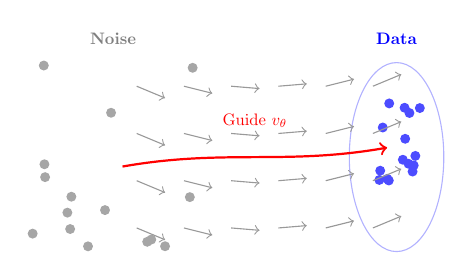
\begin{tikzpicture}[scale=0.6, transform shape]
            % Bruit (Gris) à gauche
            \node[font=\bfseries, gray] at (0, 4.5) {Noise};
            \foreach \i in {1,...,15} {
                \fill[gray!70] ({2*rand}, {2*rand + 2}) circle (3pt);
            }
            
            % Données (Bleu) à droite
            \node[font=\bfseries, blue] at (6, 4.5) {Data};
            \foreach \i in {1,...,15} {
                \fill[blue!70] ({6 + 0.5*rand}, {2 + 1.5*rand}) circle (3pt);
            }
            \draw[blue!30, thin] (6, 2) ellipse (1cm and 2cm); % Forme vague des données
            
            % Champ de vecteurs (Flèches)
            \foreach \x in {0.5, 1.5, ..., 5.5} {
                \foreach \y in {0.5, 1.5, ..., 3.5} {
                   \draw[->, black!40, thin] (\x, \y) -- ++(0.6, {0.1*(\x-3)});
                }
            }
            
            % Une trajectoire exemple
            \draw[->, red, thick] (0.2, 1.8) to[out=10, in=190] (5.8, 2.2);
            \node[red, above] at (3, 2.5) {Guide $v_\theta$};
            
        \end{tikzpicture}
    \end{columns}
\end{frame}
